
\part{Pedal de distorsión}

\section{Introducción}
Se pide implementar el circuito de un pedal de distorsión. Estos pedales son muy populares por su sonido característico y su versatilidad. En el campo del audio, la distorsión es usada normalmente para simular los efectos
de un amplificador que está saturado y se emplea principalmente con guitarras eléctricas.

El circuito genera el deseado efecto de distorsión tomando la señal de la guitarra, amplificándola y luego recortándola para simular la saturación.

La cátedra propuso un circuito al que se le hicieron modificaciones para mejorar tanto el desempeño del artefacto como su flexibilidad.

En lo que sigue se explicará el circuito inicial, luego las mejoras propuestas, posteriormente se detallará, con respaldo en simulaciones y mediciones, el comportamiento del circuito, y finalmente se realizarán algunas reseñas a modo de conclusión.

\section{Circuito propuesto por la cátedra}
Se propuso como guía un circuito básico de distorsión por recorte. Este se puede observar, con sus etapas señaladas, en la Figura \ref{fig:circuitopropuesto}.

\begin{figure}[h]
    \centering
    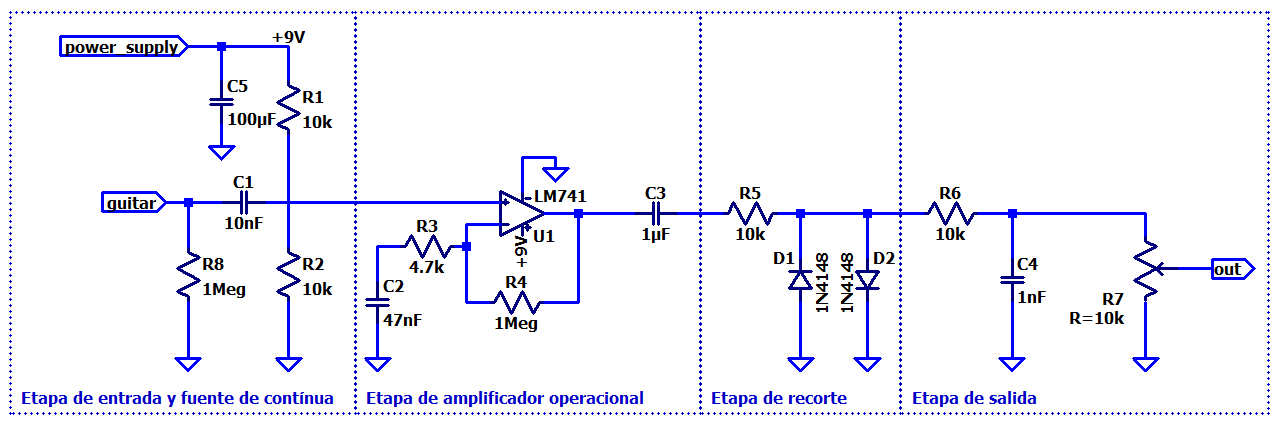
\includegraphics[width=\textwidth]{../Ex5/circuitopropuesto}
    \caption{Circuito propuesto por la cátedra}
    \label{fig:circuitopropuesto}
\end{figure}
\subsection{Etapa de entrada y fuente de contínua} \label{continuacircoriginal}
\begin{itemize}
    \item El capacitor C5 filtra las corrientes de \emph{ripple} de la fuente de 9V. A este fin, se le asigna un valor de 100 $\mu$F.
    \item Las resistencias R1 y R2 forman un divisor de tensión que pone +4,5V en la entrada no inversora del amplificador, polarizándolo. Se les da un valor moderado de 10k$\Omega$.
    \item Se coloca R8 como una resistencia de \emph{pull-down} para mantener descargado el capacitor C1 mientras el pedal no esté en uso: de este modo, se evita un sonido indeseable por un sobrepico de tensión al conectar la guitarra o presionar el interruptor. Un valor de 1M es apropiado, ya que no afecta la señal de entrada y descarga con éxito el capacitor.
    \item El capacitor C1, en conjunto con la impedancia de entrada del circuito, forma un filtro pasa-altos (léase la sección \ref{calculoimpentrada}) que elimina la corriente de contínua proveniente de la entrada, y aisla a su vez la entrada de la que pueda provenir del pedal. Se eligió el diodo 1N4004 por su disponibilidad, pero cualquier diodo sería capaz de llevar a cabo esta función.
\end{itemize}
\subsection{Etapa de amplificador operacional}\label{opampcircoriginal}
\begin{itemize}
    \item El capacitor C2, en conjunto con la resistencia R2, forman un filtro pasa-altos (léase la sección \ref{calculoganancia}). Su función es filtrar frecuencias muy bajas que pueden sobrecargar el amplificador, causando inestabilidad. Se le asigna un valor de 47nF.
    \item Se eligió el operacional LM741 por su ubicuidad y confiabilidad. Si bien su \emph{slew rate} es de 0,5$\mu$V/s y no se comporta de forma idónea en el extremo superior del espectro de frecuencias de audio (20kHz), esto no es necesariamente un problema en un pedal de distorsión: de hecho, es muy popular para esta aplicación.
    \item La resistencia R4, de 1M$\Omega$, con R3, de 4,7k$\Omega$, determinan la ganancia de la etapa, que es de 46,5dB.
    \item El capacitor C3, de 1$\mu$F sirve para filtrar cualquier corriente indeseable que surja del amplificador, desacoplando esta etapa de la siguiente.
\end{itemize}
\subsection{Etapa de recorte}
\begin{itemize}
    \item Los diodos D1 y D2 conectados a tierra recortan la señal bruscamente, generando una distorsión fuerte. Se eligió el diodo 1N4148 por su corto tiempo de recuperación, $t_{rr}=5ns$, que lo hace apto para aplicaciones \emph{fast switching}. Esta particularidad evita una distorsión indeseable (de atenuación) de la señal en esta etapa. 
    \item La resistencia R5 se coloca para limitar la corriente que atraviesa los diodos. Se eligió un valor de $10k\Omega$, pero cualquier valor entre $1k\Omega$ y el elegido hubiera sido apto.
\end{itemize}
\subsection{Etapa de salida}
\begin{itemize}
    \item El capacitor C4 y la resistencia R6 forman un filtro pasa-bajos para filtrar los armónicos demasiado agudos de la salida. Su frecuencia de corte con estos valores es de 16kHz aproximadamente.
    \item El potenciómetro R7 funciona como control de volumen, formando un divisor de tensión y dejando pasar la corriente de sobra a tierra.
\end{itemize}
\section{Cambios propuestos al circuito}
El circuito final está compuesto por cuatro etapas: la etapa de fuente de contínua, la de amplificador operacional, la de recorte, y la de tono y salida. Estas se presentan detalladamente a continuación con los cambios propuestos y se realizan los cálculos pertinentes a la designación de los valores de los componentes.
\subsection{Etapa 1: fuente de contínua}
Esta etapa alimenta al pedal de corriente contínua. El esquemático se puede observar en la Figura \ref{fig:circuitofuentecontinua}.
\begin{figure}[h]
    \centering
    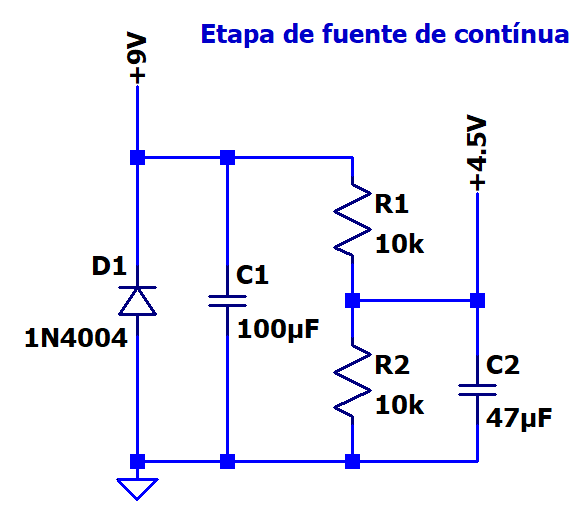
\includegraphics[width=0.5\textwidth]{../Ex5/circuitofuentecontinua}
    \caption{Circuito final: etapa de fuente de contínua}
    \label{fig:circuitofuentecontinua}
\end{figure}
\subsubsection{Mejoras propuestas}
A los componentes anteriormente señalados, se agrega:
\begin{itemize}
    \item El diodo D1, para proteger al dispositivo de un error del usuario, al conectar un adaptador con una polaridad incorrecta.
    \item El capacitor C2, para estabilizar aún más la señal de 4,5V, asegurando que tenga la menor oscilación posible.
    \end{itemize}
\subsection{Etapa 2: amplificador operacional}
Se filtra y amplifica la señal de entrada con una ganancia considerable. Se observa el diseño final de esta etapa en la Figura \ref{fig:circuitoopamp}.
\begin{figure}[h]
    \centering
    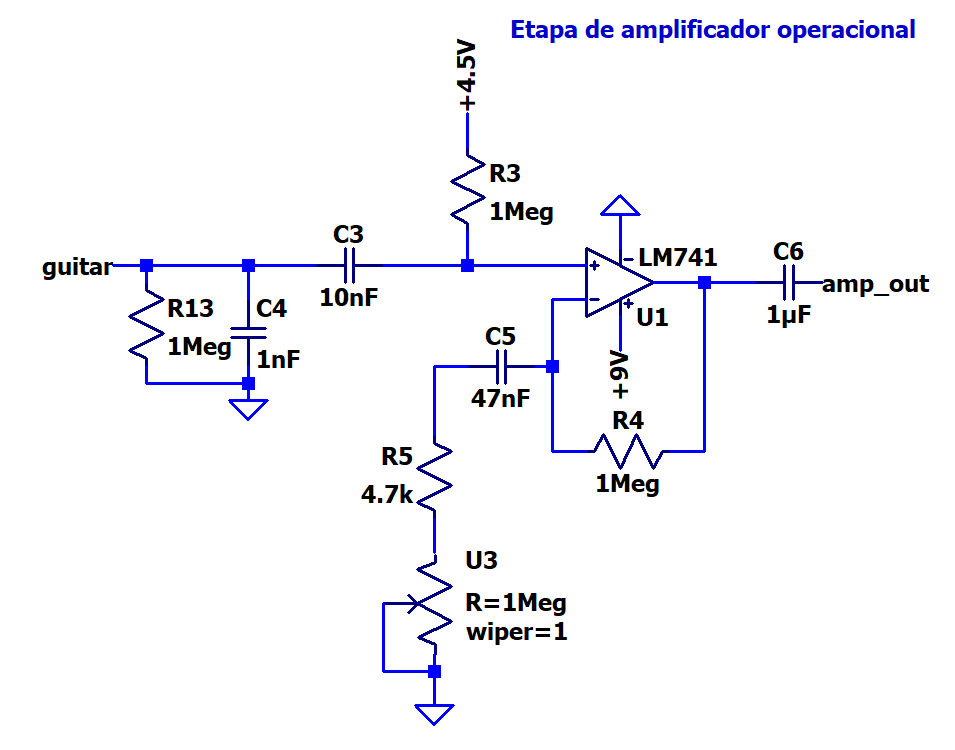
\includegraphics[width=0.8\textwidth]{../Ex5/circuitoopamp}
    \caption{Circuito final: etapa de amplificador operacional}
    \label{fig:circuitoopamp}
\end{figure}
\subsubsection{Mejoras propuestas}
A los componentes ya mencionados, se les suma:
\begin{itemize}
    \item El capacitor C4, de 1nF, que filtra las muy altas frecuencias (interferencia por radiofrecuencias) y las descargas de electricidad estática de la entrada.
    \item La resistencia R3 de 1M$\Omega$, que polariza el operacional a 4,5V y aporta a la impedancia de entrada del circuito.
    \item El potenciómetro U3, que regula la ganancia del operacional entre 46,5dB y 6dB (léase la sección \ref{calculoganancia}).
\end{itemize}
\subsubsection{Cálculo de la impedancia de entrada de la etapa} \label{calculoimpentrada}
La impedancia de entrada de esta etapa, que coincide con la del circuito, puede expresarse como:
\begin{align}
    Z_{in}=R3//Z_{Op-Amp}+Z_{4.5V},
    \qquad
    Z_{4.5V}=R1//R2
\end{align}
la impedancia de entrada del LM741, $Z_{Op-Amp}$, es de $2M\Omega$; luego,
\begin{align}
    Z_{in}=1M\Omega//2M\Omega+10k\Omega//10k\Omega=671,6k\Omega
\end{align}
Obsérvese que con este valor de $Z_{in}$, el filtro pasa-altos mencionado en la sección \ref{continuacircoriginal} tendrá una frecuencia de corte $f_{0}=\frac{1}{2\pi*Z_{in}*C3}=23.69Hz$
\subsubsection{Cálculo de la ganancia de la etapa}\label{calculoganancia}
La ganancia del operacional puede ser calculada según la siguente expresión:
\begin{align}
G_{v}=1+\frac{R4}{R5+U3}
\end{align}
Luego, tenemos que
\begin{align}
G_{min}=1+\frac{1M\Omega}{4,7k\Omega+1M\Omega}=2\\
G_{max}=1+\frac{1M\Omega}{4,7k\Omega+0\Omega}=213,7
\end{align}
lo cual nos indica una $G_{max}=46,6dB$ y una $G_{min}=6dB$.

El análisis en frecuencia de la ganancia de esta etapa para distintos valores de U3 puede observarse en la Figura \ref{fig:bodeamppote}.

\begin{figure}[h]
    \centering
    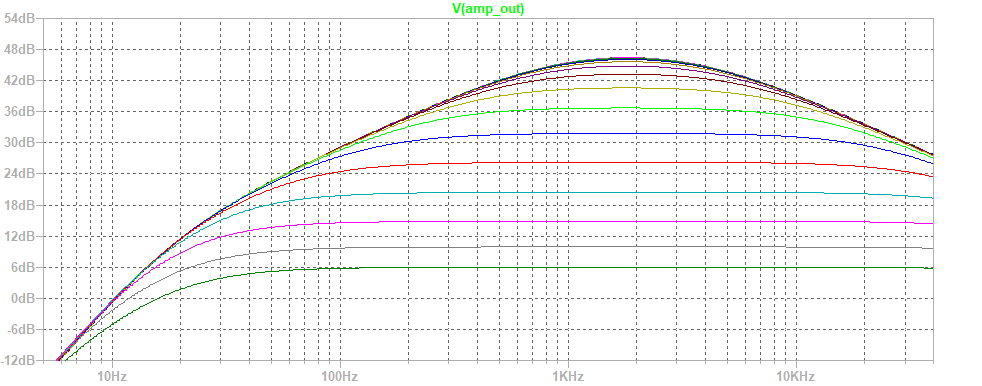
\includegraphics[width=\textwidth]{../Ex5/bodeamppote}
    \caption{Diagrama de Bode de la etapa 2 para distintos valores de U3}
    \label{fig:bodeamppote}
\end{figure}

Con estos valores, el filtro pasa-altos descripto en la sección \ref{opampcircoriginal} tendrá para $G_{max}$ una frecuencia de corte $f_{0}=\frac{1}{2\pi*4,7k\Omega*C5}=720.5Hz$, y para $G_{min}$ una frecuencia de corte $f_{0}=\frac{1}{2\pi*(1M\Omega+4,7k\Omega)*C5}=3.37Hz$.
 \subsection{Etapa 3: recorte}
 La etapa de recorte es, en conjunto con la de amplificación, la más importante en el pedal. Aquí se recorta mediante diodos conectados a tierra la señal previamente amplificada para generar el efecto de distorsión. El diseño se observa en la Figura \ref{fig:circuitorecorte}.
 \begin{figure}[h]
     \centering
     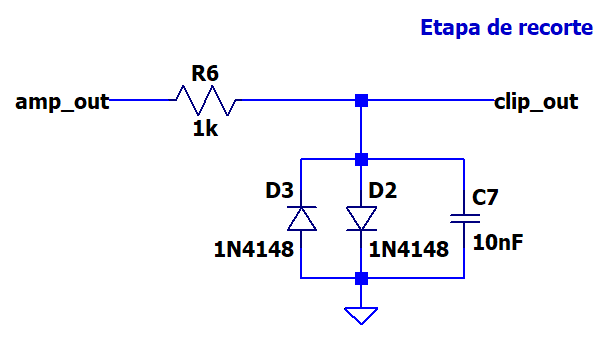
\includegraphics[width=0.7\textwidth]{../Ex5/circuitorecorte}
     \caption{Circuito final: etapa de recorte}
     \label{fig:circuitorecorte}
 \end{figure}
Como los diodos se conectan a tierra, el efecto que se produce se conoce como distorsión dura o \emph{hard clipping}: se limita la amplitud de la señal con "rectas" en $0,7V$ y $-0,7V$.

\subsubsection{Mejoras propuestas}\label{mejorasrecorte}
\begin{itemize}
    \item Se cambió el valor de la resistencia limitadora de corriente en los diodos R6 para no atenuar demasiado la señal, ya que se agregó una nueva etapa posterior a esta.
    \item Se agregó el capacitor C7, que en conjunto con la resistencia R6 funciona como un pasa-bajos con una frecuencia de corte $f_{0}=\frac{1}{2\pi*1k\Omega*10nF}=15,9kHz$. Este filtro atenúa los armónicos agudos de la señal, que no son propios del sonido de un pedal de este tipo.
\end{itemize}
\subsection{Etapa 4: control de tono}
Se agrega al pedal una etapa para regular el tono del pedal. Esta incluye un potenciómetro para control de tono y a su vez uno para control de volumen de salida. El esquemático se puede observar en la Figura \ref{fig:circuitotono}.


\begin{figure}[h]
    \centering
    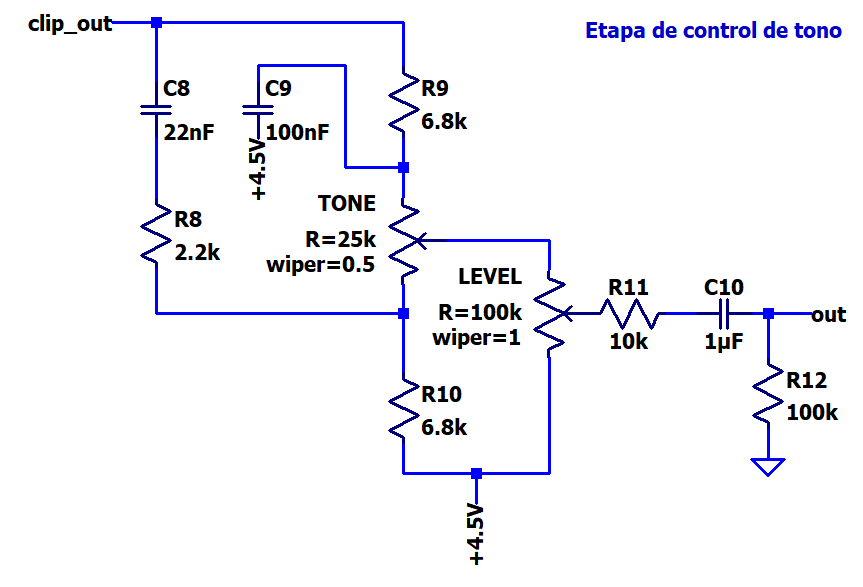
\includegraphics[width=0.7\textwidth]{../Ex5/circuitotono}
    \caption{Circuito final: etapa de control de tono}
    \label{fig:circuitotono}
\end{figure}

El circuito para esta etapa consta de dos partes. La primera comprende dos filtros en paralelo, un pasa-bajos y un pasa-altos, y un potenciómetro lineal TONE (de control de tono) para mezclar las señales provenientes de estos y generar la salida.

La segunda parte consta de un potenciómetro de control de volumen (también lineal por indisponibilidad de potenciómetros logarítmicos) que descarga parte de la señal a tierra, en conjunto con un filtro pasa-altos con una frecuencia de corte  $f_{0}=\frac{1}{2\pi*100k\Omega*1\mu F}=1,6Hz$, que filtra la componente de contínua de la señal de salida.

\subsubsection{Funcionamiento de la etapa en frecuencias}\label{frecuenciatono}
En la Figura \ref{fig:bodetono} se muestra la respuesta de la etapa simulada en \emph{LTSpice} para distintas frecuencias de entrada y para distintos valores de TONE. Se puede observar en verde la curva de ganancia para cuando el circuito funciona como un pasa-bajos, es decir, cuando TONE está al mínimo, y en azul la curva para cuando TONE está al máximo y la etapa es un pasa-altos. Las curvas restantes representan la salida para valores intermedios del potenciómetro.

\begin{figure}[h]
    \centering
    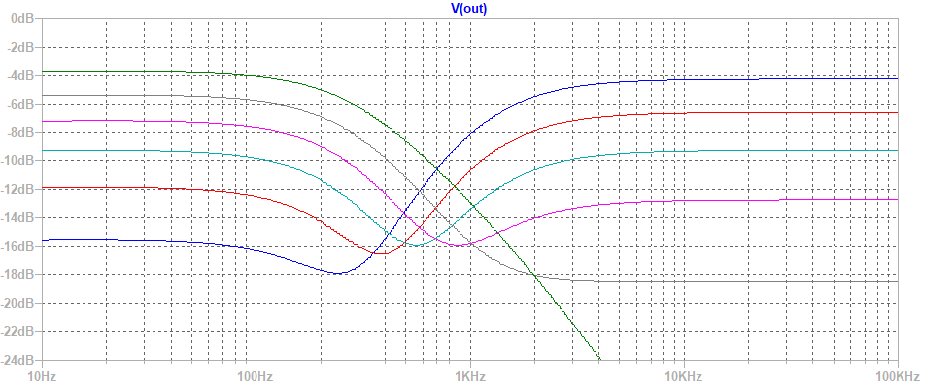
\includegraphics[width=\textwidth]{../Ex5/bodetono}
    \caption{Diagrama de Bode para la etapa 4 para distintos valores de TONE}
    \label{fig:bodetono}
\end{figure}

Cabe destacar que se calcularon los valores para que cuando el potenciómetro TONE, que es lineal, esté en posición media, se atenúen las señales de frecuencias cercanas a $1kHz$.

\section{Comportamiento del circuito}
A continuación se muestra el análisis del comportamiento del circuito acompañado de las simulaciones en \emph{LTSpice} y las mediciones correspondientes.

Si bien las mediciones se condicen con las simulaciones en una medida considerable, existen ciertas discrepancias: estas se deben a que se trabajó con señales de entrada con tensiones del orden de las decenas de mV, las correspondientes a la salida de una guitarra real: esto significa que el ruido del laboratorio tiene una influencia notable.

Se tiene en cuenta que para el análisis en frecuencias de un circuito lineal (ignorando los diodos) la tensión de entrada no tiene demasiada importancia; sin embargo, la ganancia del amplificador operacional (46,5dB) es tal que no pudieron usarse señales de entrada muy diferentes a las mencionadas para evitar efectos de recorte, que sí hubieran alterado el análisis, en el mismo.

\subsection{A la salida del amplificador operacional}
En la Figura \ref{fig:bodeopamp} se puede observar la ganancia de la etapa de amplificador operacional para distintas frecuencias de entrada. Si bien el rango analizado excede el espectro de audio, resulta interesante analizar el comportamiento más allá del mismo.

\begin{figure}[h]
    \centering
    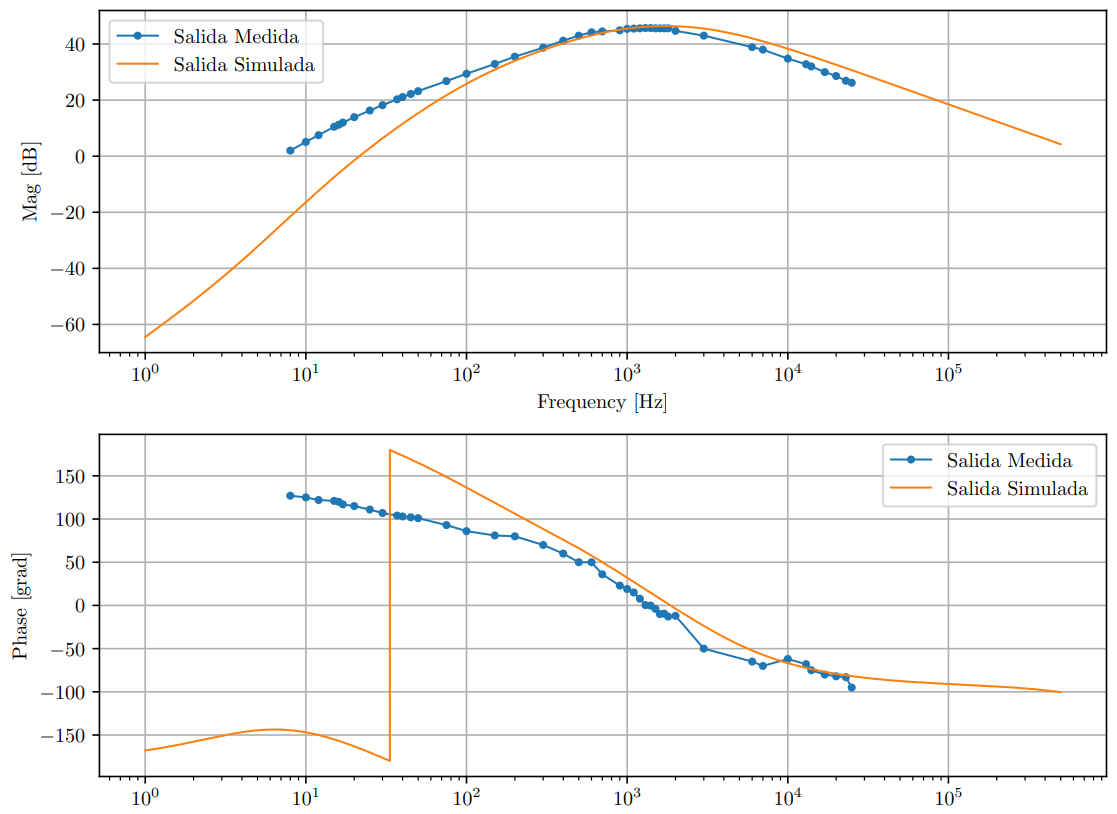
\includegraphics[width=0.8\textwidth]{../Ex5/bodeopamp}
    \caption{Diagrama de Bode para la etapa de Op-Amp}
    \label{fig:bodeopamp}
\end{figure}

Se puede observar que se presenta la máxima ganancia de 46,5dB mencionada para el orden de frecuencias de 1kHz. También se puede ver que se amplifican las frecuencias del espectro de audio, filtrando las muy bajas, gracias al filtro de 23Hz en la entrada (léase la sección \ref{continuacircoriginal}).

\subsection{A la salida de audio}
En la Figura \ref{fig:bodepedal} se puede observar la ganancia del pedal completo para distintas frecuencias de entrada.

\begin{figure}[h]
    \centering
    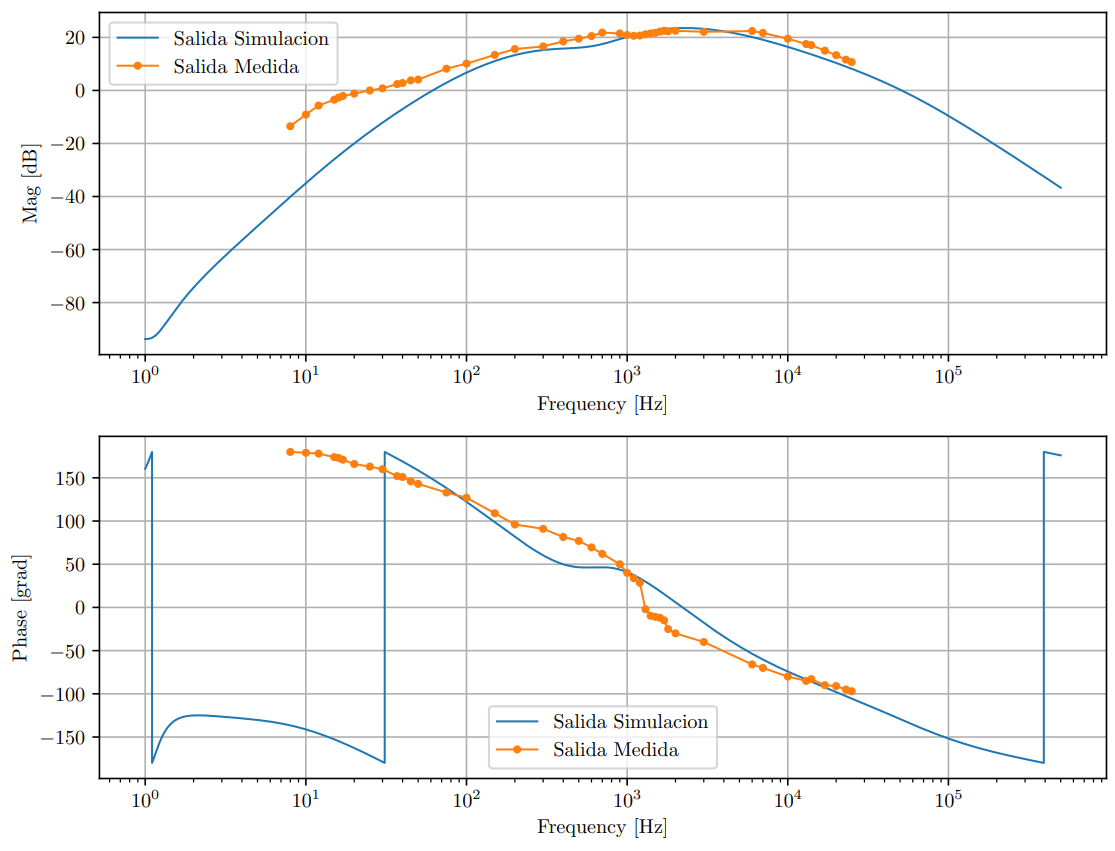
\includegraphics[width=0.8\textwidth]{../Ex5/bodepedal}
    \caption{Diagrama de Bode para el pedal completo}
    \label{fig:bodepedal}
\end{figure}


Cabe destacar que este análisis (simulaciones y medición en el laboratorio) se realizó para los valores máximos de transferencia de la etapa de amplificador operacional (es decir, con U3 en $0\Omega$), el potenciómetro LEVEL al máximo volumen, y el control de tono al valor medio mencionado en la sección \ref{frecuenciatono}.

Nótese que la señal comienza a caer a partir de 1kHz y su caída se acentúa a partir los aproximadamente 17kHz, debido al pasa-bajos mencionado en la sección \ref{mejorasrecorte}.

Puede observarse una atenuación de aproximadamente 20dB respecto de la salida de la etapa del amplificador operacional (ver Figura \ref{bodeopamp}). Esto se debe a que la etapa 4 (de control de tono) atenúa la señal en esa magnitud. Esto no representa un problema, pues aún con esta caída de tensión la salida presenta una tensión de aproximadamente $400mV_{pp}$, la cual es aceptable para una interfaz de audio.

Puede también observarse un área de interés en la vecindad de $f=1kHz$, donde la señal se ve puntualmente atenuada. Esto se debe a que el potenciómetro de control de tono está en una posición media, y se produce el efecto explicado en la sección \ref{frecuenciatono}.

\section{Conclusión}
Se diseñó, simuló, construyó y midió un pedal de distorsión para guitarra. Se investigó sobre y experimentó con amplificadores operacionales, se analizaron las ventajas y desventajas para esta aplicación de distintos modelos, y resultó interesante utilizar uno que no resultaría idealmente apto, por características como su \emph{slew rate}, pero que debido a la naturaleza de la aplicación, puede usarse de todos modos.

Se investigaron también los distintos tipos de diodos, y se encontró uno que se adaptó al uso que se le quería dar.

Se analizó el funcionamiento del producto final y se lo encontró apto para el uso al que se destina.
